\subsection{Verteilungsfunktionen}

In diesem Abschnitt werden wir uns mit einer wichtigen Funktion beschäftigen, die für jede reelle Zufallsvariable existiert.

\begin{Definition}{(Verteilungsfunktion)}
Sei $X$ eine reelle Zufallsvariable. Durch 
\[F_X: \mathbb{R} \rightarrow [0, 1]: x \mapsto F_X(x) := \mathbb{P}(X \leq x)\]
ist die \textit{Verteilungsfunktion} definiert.
\end{Definition}

Wir werden nun einige Eigenschaften von Verteilungsfunktionen beweisen.

\begin{Satz}{(Eigenschaften Verteilungsfunktion)}
\hypertarget{Satz:EigVertFun}{}Sei $(\Omega, \mathscr{A}, \mathbb{P})$ ein Wahrscheinlichkeitsraum und $X$ eine reelle Zufallsvariable. Die Verteilungsfunktion $F_X$ hat dann die folgenden Eigenschaften.
\begin{enumerate}[label=\textup{(\roman*)}]
\item $F_X$ ist rechtsseitig stetig.
\item $F_X$ ist monoton wachsend.
\item $\lim_{x \rightarrow -\infty} F_X(x) = 0$.
\item $\lim_{x \rightarrow \infty} F_X(x) = 1$.
\end{enumerate}
\end{Satz}

\newpage

\begin{Beweis}{}
Zu (i):\\
Sei $x \in \mathbb{R}$ beliebig und $(x_n)_{n \in \mathbb{N}_0}$ eine monoton fallende Folge mit Grenzwert $x$. Betrachte
\begin{align*}
\lim_{n \rightarrow \infty} F_X(x) &= \lim_{n \rightarrow \infty} \mathbb{P}(X \leq x_n)~.
\intertext{Da $\mathbb{P}$ als Wahrscheinlichkeitsmaß insbesondere stetig von oben ist, kann man den Limes reinziehen und erhält}
&= \mathbb{P}(X \leq x)\\
&= F_X(x)~.
\end{align*}
Somit ist $F_X$ rechtsseitig stetig.\\

Zu (ii):\\
Sei $x_1 \leq x_2$ aus $\mathbb{R}$. Betrachte
\begin{align*}
F_X(x_2) - F_X(x_1) &= \mathbb{P}(X \leq x_2) - \mathbb{P}(X \leq x_1)\\
&= \int_\mathbb{R} \indi_{(-\infty, x_2]} \d \mathbb{P}_X - \int_\mathbb{R} \indi_{(-\infty, x_2]} \d \mathbb{P}_X~.
\intertext{Mit der Linearität des Integrals gilt}
&= \int_\mathbb{R} \indi_{(-\infty, x_2]} - \indi_{(-\infty, x_1]} \d \mathbb{P}_X~.
\intertext{Wir werden gleich sehen, dass folgenden Umformung eine Identität ist}
&= \int_\mathbb{R} \indi_{[x_1, x_2]} \d \mathbb{P}_X\\
&= \mathbb{P}(X \in [x_1, x_2]) \geq 0~,
\end{align*}
dank (M2). Umformen liefert
\[F_X(x_2) \geq F_X(x_1)~.\]
Zum Beweis der oben verwendeten Identität, betrachte die folgende Tabelle:

\begin{center}
\renewcommand{\arraystretch}{1.5}
\begin{tabularx}{\linewidth}{c | c c c c}
& $\indi_{(-\infty, x_1]}(x)$ & $\indi_{(-\infty, x_2]}(x)$ & $\indi_{(-\infty, x_2]}(x) - \indi_{(-\infty, x_1]}(x)$ & $\indi_{[x_1, x_2]}(x)$\\
\hline
$x \in (-\infty, x_1]$ & $1$ & $1$ & $0$ & $0$\\
$x \in (x_1, x_2)$ & $0$ & $1$ & $1$ & $1$\\
$x \in [x_2, \infty)$ & $0$ & $0$ & $0$ & $0$
\end{tabularx}
\end{center}

Da die letzten beiden Spalten immer übereinstimmen gilt für alle $x \in \mathbb{R}$
\[\indi_{(-\infty, x_2]}(x) - \indi_{(-\infty, x_1]}(x) = \indi_{[x_1, x_2]}(x)~.\]

Zu (iii):\\
Betrachte
\begin{align*}
\lim_{x \rightarrow -\infty} F_X(x) &= \lim_{x \rightarrow -\infty} \mathbb{P}(X \leq x)\\
&= \lim_{x \rightarrow -\infty} \int \indi_{(-\infty, x]} \d \mathbb{P}_X~.
\intertext{Mit dem Satz von Lebesgue können wir Integration und Limesbildung vertauschen und es gilt}
&= \int \lim_{x \rightarrow -\infty} \indi_{(-\infty, x]} \d \mathbb{P}_X\\
&= \int \indi_{\emptyset} \d \mathbb{P}_X \\
&= \mathbb{P}_X(\emptyset) = 0~,
\end{align*}
da $\mathbb{P}_X$ als Maß insbesondere nulltreu ist.\\

Zu (iv):\\
Betrachte
\begin{align*}
\lim_{x \rightarrow \infty} F_X(x) &= \lim_{x \rightarrow \infty} \mathbb{P}(X \leq x)\\
&= \lim_{x \rightarrow \infty} \int \indi_{(-\infty, x]} \d \mathbb{P}_X~.
\intertext{Mit dem Satz von Lebesgue können wir Integration und Limesbildung vertauschen und es gilt}
&= \int \lim_{x \rightarrow \infty} \indi_{(-\infty, x]} \d \mathbb{P}_X\\
&= \int \indi_\mathbb{R} \d \mathbb{P}_X \\
&= \mathbb{P}_X(\mathbb{R}) = 1~,
\end{align*}
da $\mathbb{P}_X$ ein Wahrscheinlichkeitsmaß ist.
\end{Beweis}

\vspace*{\baselineskip}

Wir werden nun eine Möglichkeit finden, diese Verteilungsfunktion auf einfache Weise zu berechnen.

\begin{Bemerkung}{(Berechnung der Verteilungsfunktion)}
\hypertarget{Verteilungsfunktion}{} Sei $X$ eine stetige Zufallsvariable mit Dichte $\varphi$. Dann gilt dank dem \hyperlink{Kor:Dichtekorollar}{\blue{Dichtekorollar}}
\begin{align*}
F_X(x) &= \mathbb{P}(X \leq x)\\
&= \int \indi_{\{\omega: X(\omega) \leq x\}}(\omega) \d \mathbb{P}(\omega)\\
&= \int \indi_{X \in (- \infty, x]} \d \mathbb{P}\\
&= \int \indi_{(-\infty, x]} \varphi \d x\\
&= \int_{-\infty}^x \varphi \d x~.
\end{align*}
Wir können also einfach die Einsfunktion bis zum Wert $x$ integrieren. Für diskrete Zufallsvariablen berechnen wir
\[F_X(x) = \sum_{n = 0}^{\lfloor x \rfloor} \varphi(n)~.\]
Es sei an dieser Stelle nochmal erwähnt, dass die Verteilungsfunktion eine Funktion von $\mathbb{R}$ nach $[0, 1]$ ist. Wir können also jeden reellen Wert einsetzen und nicht nur Werte, die $X$ annehmen kann. Deshalb müssen wir hier die Abrundungsfunktion $\lfloor \cdot \rfloor$ verwenden.
\end{Bemerkung}

\newpage

Wir können nun eine Methode schreiben, welche zu einer Zufallsvariable die Verteilungsfunktion berechnet.

\begin{Code}{(\lstinline|distribution_function|)}
Die Berechnung der Verteilungsfunktion ist leider etwas komplizierter. Aufgrund dessen müssen wir hier wieder die verschiedenen Typen unterscheiden.
\begin{enumerate}[label=(\roman*)]
\item Für finite Zufallsvariablen gilt
\begin{lstlisting}
def distribution_function(self):
    sortable = True
    keys = list(self.density.keys())
    for key in keys:
        if isinstance(key, sym.Symbol):
            print('WARNING: Can\'t sort values.')
            sortable = False
            break
    if sortable:
        keys = sorted(keys)
    cumulative_probability = self.density[keys[0]]
    distribution_function = {keys[0]: cumulative_probability}
    keys.pop(0)
    for key in keys:
        cumulative_probability += self.density[key]
        distribution_function.update({key: cumulative_probability})
    return distribution_function
\end{lstlisting}
Im ersten Schritt wird überprüft, ob die Werte der Zufallsvariable, also die Keys des Dictionaries, sortierbar sind. Sind sie nicht sortierbar, so wird die Verteilungsfunktion aufgrund der gegebenen Reihenfolge berechnet. Nun wird die erste kumulierte Wahrscheinlichkeit festgelegt und diese mit dem entsprechenden Wert der Zufallsvariable der Verteilungsfunktion hinzugefügt. Zuletzt wird dieser Wert aus der Liste der Werte entfernt. Im nächsten Schritt wird über alle anderen Werte iteriert. Dazu wird die Wahrscheinlichkeit für den entsprechenden Wert der kumulierte Wahrscheinlichkeit hinzuaddiert und das Dictionary um das entsprechende Paar erweitert. Man erhält am Schluss also ein Dictionary. Die Keys sind die ersten Werte, ab denen die sich im Value befindende kumulierte Wahrscheinlichkeit angenommen wird. Dies sind also jeweils nach links geschlossene halboffene Intervalle. Insbesondere ist auf dem offenen Intervall von $- \infty$ bis zum ersten Wert die kumulierte Wahrscheinlichkeit (implizit) null. 

\item Für diskrete Zufallsvariablen gilt
\begin{lstlisting}
def distribution_function(self, value=None):
    if value == None:
        t = sym.Symbol('t', real=True)
        upper = sym.Min(self.supp[1], sym.floor(t))
        distribution_function = self.integrate_random_variable(sym.Integer(1), upper=upper)
        return distribution_function
    else:
        value = sym.sympify(value)
        upper = sym.Min(self.supp[1], sym.floor(value))
        distribution_function = self.integrate_random_variable(sym.Integer(1), upper=upper)
        distribution_function = float(distribution_function.evalf())
        return distribution_function
\end{lstlisting}
Die Berechnung der Verteilungsfunktion für diskrete Zufallsvariablen läuft über zwei verschiedene Arten ab. Ruft man die Methode ohne weiteres Argument auf, so ergibt sich die obere Grenze über die Abrundungsfunktion $\lfloor t \rfloor$ und das Minimum mit der oberen Schranke für den Wertebereich. Anschließend wird über die Eins summiert bis zu dieser oberen Grenze.

\newpage

Verwendet man als Argument eine Zahl, so wird diese ebenfalls abgerundet und das Minimum mit der oberen Grenze gebildet. Auch hier wird die Summe über die Eins gebildet. Anders als zuvor wird dieser Wert nun evaluiert und in eine Gleitkommazahl umgewandelt. Diese zweite Methode wird später für den \hyperlink{Code:PlotDistr}{\blue{Plot der Verteilungsfunktion}} und die \hyperlink{Sec:Sim}{\blue{Simulation}} wichtig.

\item Für stetige Zufallsvariablen gilt
\begin{lstlisting}
def distribution_function(self):
    t = sym.Symbol('t', real=True)
    distribution_function = self.integrate_random_variable(sym.Integer(1), upper=t)
    return distribution_function
\end{lstlisting}
Diese Berechnung ist viel näher an der Definition der Verteilungsfunktion. Dabei wird die Einsfunktion mithilfe der Integrationsmethode integriert, wobei die obere Grenze die Variable der Verteilungsfunktion ist.
\end{enumerate}
\end{Code}

\vspace*{-\medskipamount}

Wir können nun einige Verteilungsfunktionen berechnen.

\begin{Beispiel}{(Verteilungsfunktionen)}
\hypertarget{Bsp:VertFun}{}Da diskrete Zufallsvariablen Treppenfunktionen als Verteilungsfunktionen haben und sich die Summen nicht weiter zusammenfassen lassen, werden wir nur finite und stetige Beispiele betrachten.
\begin{enumerate}[label=(\roman*)]
\item Sei $X \sim \Ber(p)$ mit $p \in (0, 1)$ Bernoulli-verteilt. Wir finden die folgende Verteilungsfunktion
\[F_X(x) = \begin{cases}
0 &, x \in (- \infty, 0)\\
1 - p &, x \in [0, 1)\\
1 &, x \in [1, \infty)~.
\end{cases}\]
Mittels
\begin{lstlisting}[numbers=left, numberstyle=\tiny\color{codegray}]
n = sym.Symbol('n', integer=True,positive=True)
p = sym.Symbol('p', real=True, positive=True)
density = {1: p, 0: 1 - p}
rv = RandomVariableFinite(density, n)
distribution_function = rv.distribution_function()
\end{lstlisting}
erhalten wir \lstinline|{0: 1 - p, 1: 1}|. Dies entspricht genau dem oben Berechneten.
\item Sei $X \sim \Exp(\lambda)$ mit $\lambda > 0$ exponentialverteilt. Für $x \geq 0$ betrachten wir deshalb
\begin{align*}
F_X(x) &= \mathbb{P}(X \leq x)\\
&= \int_{-\infty}^x \lambda \exp(- \lambda x) \indi_{[0, \infty)}(x) \d x\\
&= \int_0^x \lambda \exp(- \lambda x) \d x\\
&= \left[ - \exp(- \lambda x) \right]_0^x\\
&= - \exp(- \lambda x) + 1~.
\end{align*}
Nach den \hyperlink{Satz:EigVertFun}{\blue{Eigenschaften der Verteilungsfunktion}} ist für $x < 0$ dann $F_X(x) = 0$. Um den oberen Teil der Verteilungsfunkion mit SymPy auszurechnen, verwenden wir
\begin{lstlisting}[numbers=left, numberstyle=\tiny\color{codegray}]
x = sym.Symbol('x', real=True)
lamda = sym.Symbol('lambda', real=True, positive=True)
density = lamda * sym.exp(- lamda * x)
rv = RandomVariableContinuous(density, x, [sym.Integer(0), sym.oo])
distribution_function = rv.distribution_function()
\end{lstlisting}
und erhalten \lstinline|1 - exp(-lambda*t)| wie oben.
\item Sei $X$ auf $[0, 1]$ stetig gleichverteilt. Betrachte zu $x \in [0, 1]$
\begin{align*}
F_X(x) &= \mathbb{P}(X \leq x)\\
&= \int_{-\infty}^x \indi_{[0, 1]}(x) \d x\\
&= \int_0^x 1 \d x\\
&= \left[ x \right]_0^x\\
&= x~.
\end{align*}
Nach den \hyperlink{Satz:EigVertFun}{\blue{Eigenschaften der Verteilungsfunktion}} ist $F_X(x) = 0$ für $x < 0$ und $F(x) = 1$ für $x > 1$. Mittels
\begin{lstlisting}[numbers=left, numberstyle=\tiny\color{codegray}]
x = sym.Symbol('x', real=True)
density = sym.Integer(1)
rv = RandomVariableContinuous(density, x, [sym.Integer(0), sym.Integer(1)])
distribution_function = rv.distribution_function()
\end{lstlisting}
erhalten wir \lstinline|Min(1, t)|, was gleichbedeutend ist mit Obigem. Wir können SymPy bei der Integration leider nicht mitteilen, dass die obere Grenze kleiner eins ist, weshalb es zu diesem Minimum kommt.
\end{enumerate}
Vor allem diese letzte Verteilungsfunktion wird bei der Simulation noch sehr wichtig werden. Zu den anderen Beispielen werden wir die Verteilungsfunktion gleich noch visualisieren.
\end{Beispiel}

Wie bei den Dichtefunktionen könnte man sich hier natürlich auch eine Visualisierung wünschen. Diese ist im Folgenden beschrieben.

\begin{Code}{(\lstinline|plot_distribution_function|)}
\hypertarget{Code:PlotDistr}{}Wie bei \hyperlink{Code:PlotDensity}{\blue{\lstinline|plot_density|}} müssen wir hier die verschiedenen Typen von Zufallsvariablen unterscheiden. Teile der Methoden wurden dort schon erläutert, weshalb diese hier nicht wiederholt werden.
\begin{enumerate}[label=(\roman*)]
\item Für finite Zufallsvariablen gilt
\begin{lstlisting}
def plot_distribution_function(self, show=True, use_latex=True):
    if self._test_for_symbols():
        return
    distribution_function = self.distribution_function()
    keys = list(distribution_function.keys())
    min_value = min(keys)
    max_value = max(keys)
    distance = max_value - min_value
    lower = min_value - 0.1 * distance
    upper = max_value + 0.1 * distance
    if use_latex:
        plt.rc('text', usetex=True)
    fig, ax = plt.subplots()
    ax.set_xlabel(f'${sym.latex(self.variable)}$')
    ax.set_ylabel('Distribution function')
    ax.hlines(y=0, xmin=lower, xmax=min_value, color='tab:blue', linewidth=2)
    ax.hlines(y=1, xmin=max_value, xmax=upper, color='tab:blue',linewidth=2)
    for num, key in enumerate(keys):
        if num < len(keys) - 1:
            ax.hlines(y=distribution_function[key], xmin=keys[num], xmax=keys[num+1], color='tab:blue', linewidth=2)
    if show:
        plt.show()
    else:
        return fig, ax
\end{lstlisting}
Zuerst lassen wir mit der gerade definierten \lstinline|distribution_function|-Methode die Verteilungsfunktion berechnen. Zu den $x$-Werten der Sprungstellen berechnen wir nun Minimum, Maximum sowie deren Abstand. Um die linke und rechte Grenze des Plots zu bestimmen, geben wir jeweils $10 \%$ der Länge als Puffer dazu. Als nächstes bilden wir zwei horizontale Linien auf den Höhen Null und Eins. Wir iterieren nun über alle restlichen Werte und fügen die entsprechenden Horizontalen ein.

\item Für diskrete Zufallsvariablen gilt
\begin{lstlisting}
def plot_distribution_function(self, lower=0, upper=10, show=True, use_latex=True):
    if self._test_for_symbols():
        return
    lower = int(np.floor(lower))
    upper = int(np.ceil(upper))
    if use_latex:
        plt.rc('text', usetex=True)
    fig, ax = plt.subplots()
    ax.set_xlabel(f'${sym.latex(self.variable)}$')
    ax.set_ylabel('Distribution function')
    for num in range(lower, upper + 1):
        propability = self.distribution_function(value=num)
        ax.hlines(y=propability, xmin=num - 1, xmax=num, color='tab:blue', linewidth=2)
    if show:
        plt.show()
    else:
        return fig, ax
\end{lstlisting}
Da wir bei dieser Methode eine untere und obere Grenze selbst wählen können, müssen wir in einem ersten Schritt diese entsprechend runden, um später sinnvoll iterieren zu können. Standardmäßig wird die Verteilungsfunktion auf dem Intervall $[0, 10]$ geplottet. Wir iterieren über alle ganzen Zahlen von der unteren Grenze bis zur oberen Grenze eingeschlossen. Die kumulierte Wahrscheinlichkeit erhalten wir von der \lstinline|distribution_function|-Methode im numerischen Modus. Damit können wir dann die passenden Horizontalen plotten.

\item Für stetige Zufallsvariablen gilt
\begin{lstlisting}
def plot_distribution_function(self, lower=-5, upper=5, numpoints=100, show=True, use_latex=True):
    if self._test_for_symbols():
        return
    distribution_function = self.distribution_function()
    t = sym.Symbol('t', real=True)
    x_values = np.linspace(lower, upper, num=numpoints)
    y_values = []
    for x_value in x_values:
        if x_value < self.supp[0]:
            y_value = 0
        elif x_value > self.supp[1]:
            y_value = 1
        else:
            y_value = float(distribution_function.subs(t, x_value).evalf())
        y_values.append(y_value)
    if use_latex:
        plt.rc('text', usetex=True)
    fig, ax = plt.subplots()
    ax.set_xlabel(f'${sym.latex(self.variable)}$')
    ax.set_ylabel('Distribution function')
    ax.plot(x_values, y_values)
    if show:
        plt.show()
    else:
        return fig, ax
\end{lstlisting}
Als erstes lassen wir die Verteilungsfunktion berechnen. Anschließen bestimmen wir mit NumPy äquidistante $x$-Werte zwischen der unteren und oberen Grenze. Diese lassen sich beliebig ändern. Standardmäßig wird das Intervall $[-5, 5]$ geplottet. Um die kumulierte Wahrscheinlichkeit zu bestimmen iterieren wir über alle $x$-Werte. Zuerst wird überprüft, ob dieser Wert kleiner ist als der Träger. In diesem Fall verschwindet die kumulierte Wahrscheinlichkeit. Ist der Wert größer als der Träger, so ist diese eins. Ansonsten setzen wir in die Verteilungsfunktion den $x$-Wert ein und werten diese dort aus. Zum Schluss plotten wir unsere so berechneten $x$- und $y$-Werte.
\end{enumerate}
An dieser Stelle sei noch darauf hingewiesen, dass die Verteilungsfunktion strenggenommen rechtsseitig stetig ist und wir dies an den Anfängen und Enden der Linien entsprechend kennzeichnen könnten. Darauf wurde verzichtet, um die Plots übersichtlicher zu gestalten.
\end{Code}

Im folgenden Beispiel werden wir uns zu den Beispielen, für die wir \hyperlink{Bsp:DichteBild}{\blue{bereits}} die Dichtefunktion visualisiert haben, auch die Verteilungsfunktion plotten.

\begin{Beispiel}{(Plots von Verteilungsfunktionen)}
Auf Änderungen am Plot wollen wir an dieser Stelle verzichten. Wir fügen \lstinline|rv.plot_distribution_function| an die entsprechenden Codeschnipsel an.\\
\begin{minipage}{0.5\linewidth}
\begin{figure}[H]
\begin{center}
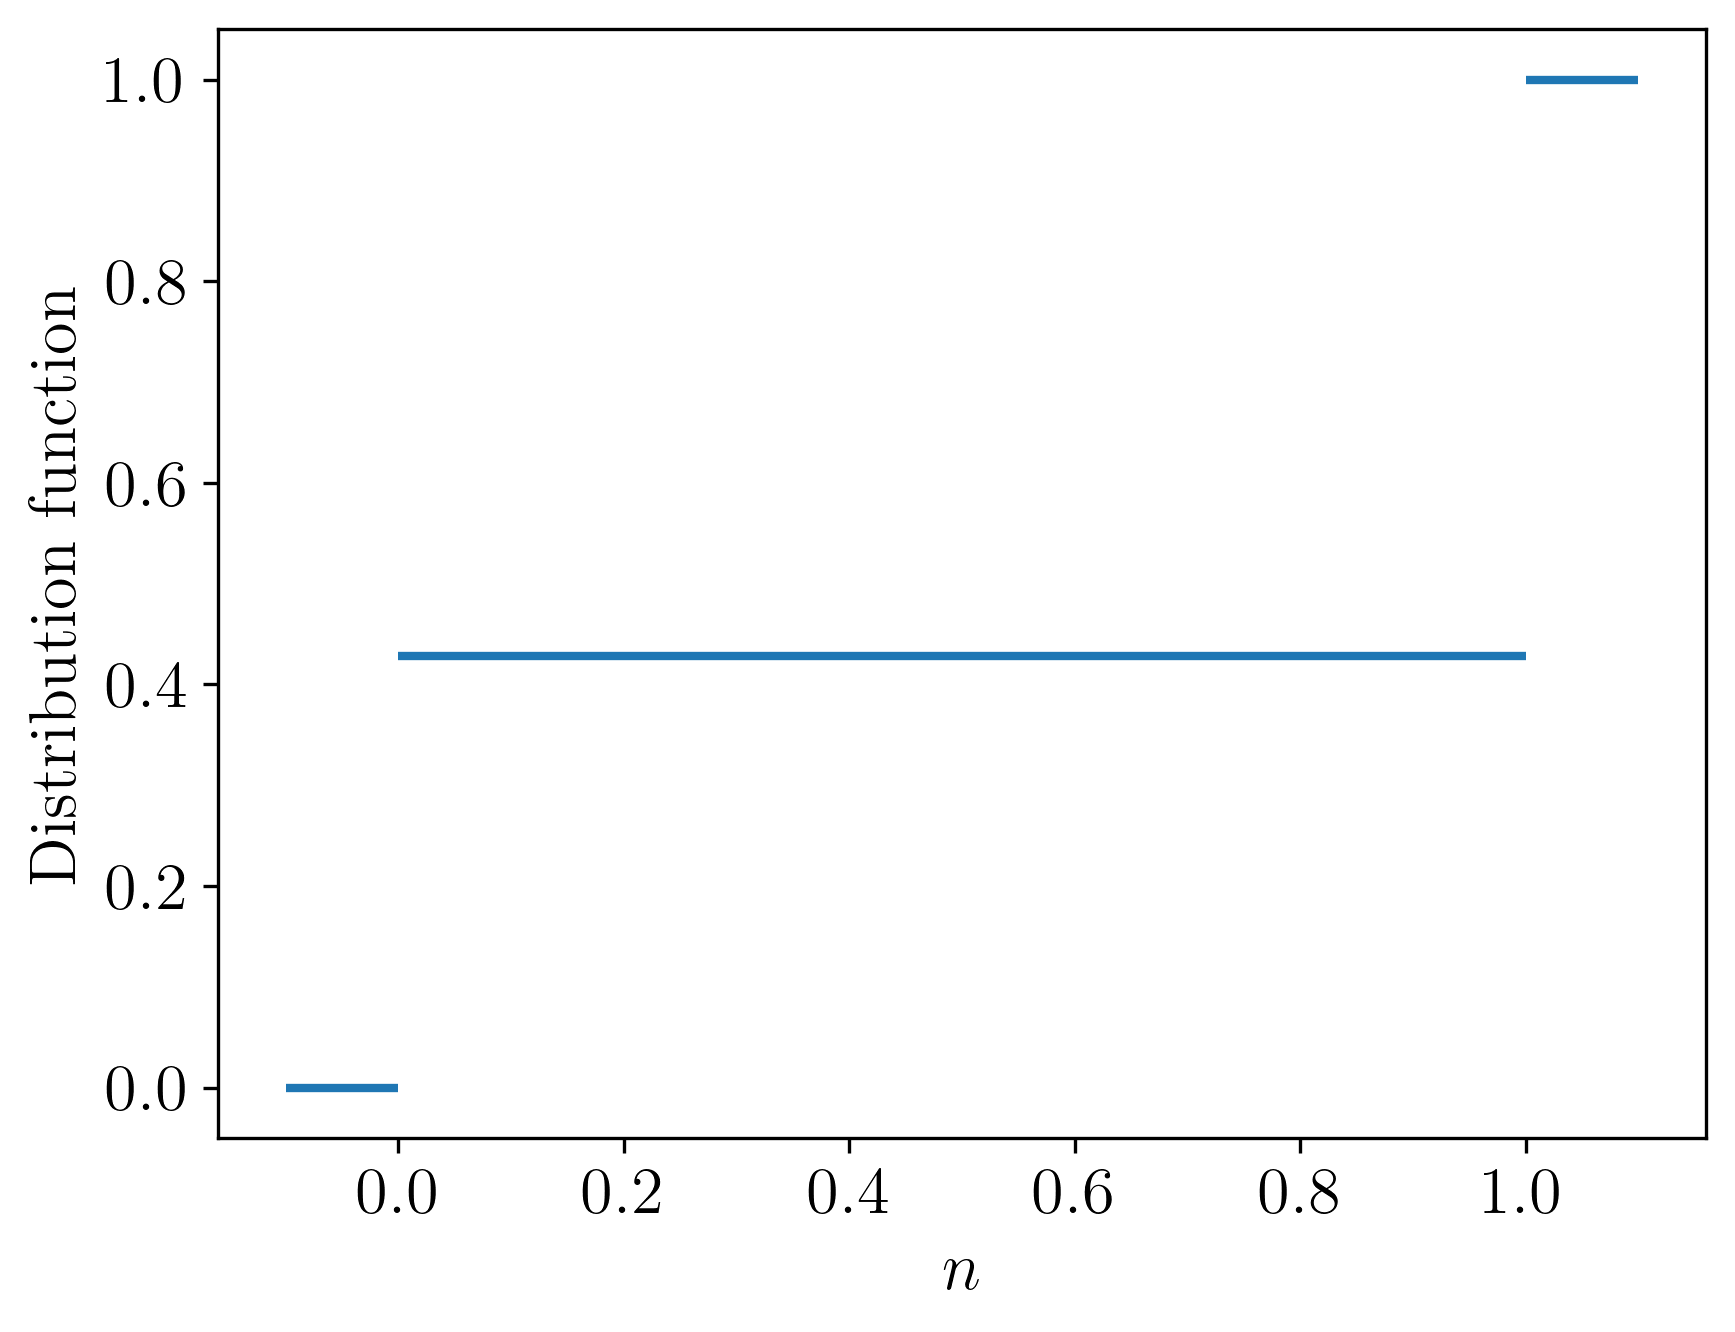
\includegraphics[width=.9\linewidth]{./Section/Grundlegende Begriffe/Verteilungsfunktion Bernoulli.png}
\vspace*{-.3\baselineskip}
\caption{\centering Verteilungsfunktion einer $\Ber(4/7)$-Verteilung}
\vspace*{-.3\baselineskip}
\end{center}
\end{figure}
\end{minipage}
\begin{minipage}{0.5\linewidth}
\begin{figure}[H]
\begin{center}
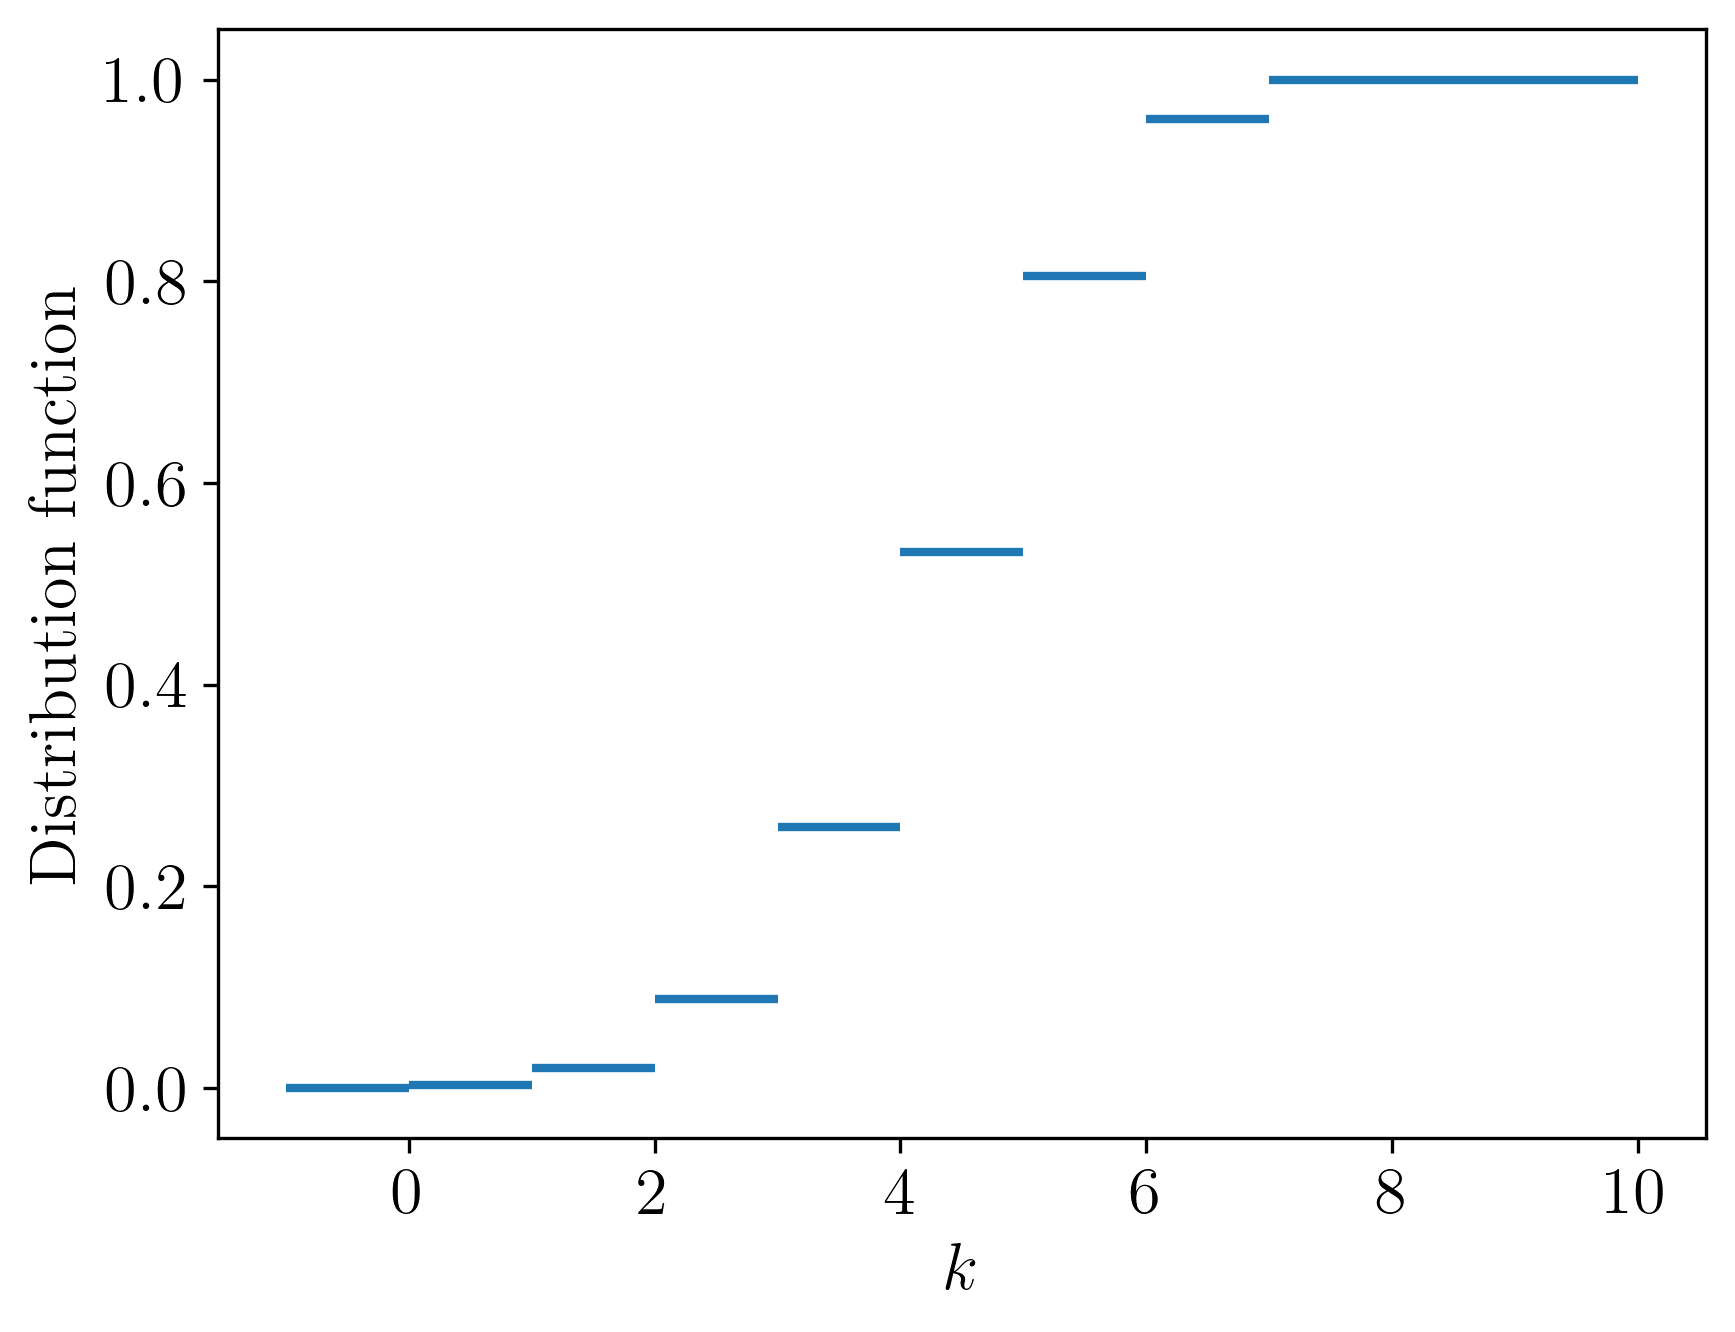
\includegraphics[width=.9\linewidth]{./Section/Grundlegende Begriffe/Verteilungsfunktion Binomial.png}
\vspace*{-.3\baselineskip}
\caption{\centering Verteilungsfunktion einer $\Bin(8, 2/3)$-Verteilung}
\vspace*{-.3\baselineskip}
\end{center}
\end{figure}
\end{minipage}
\vspace*{-\baselineskip}

\begin{minipage}{0.5\linewidth}
\begin{figure}[H]
\begin{center}
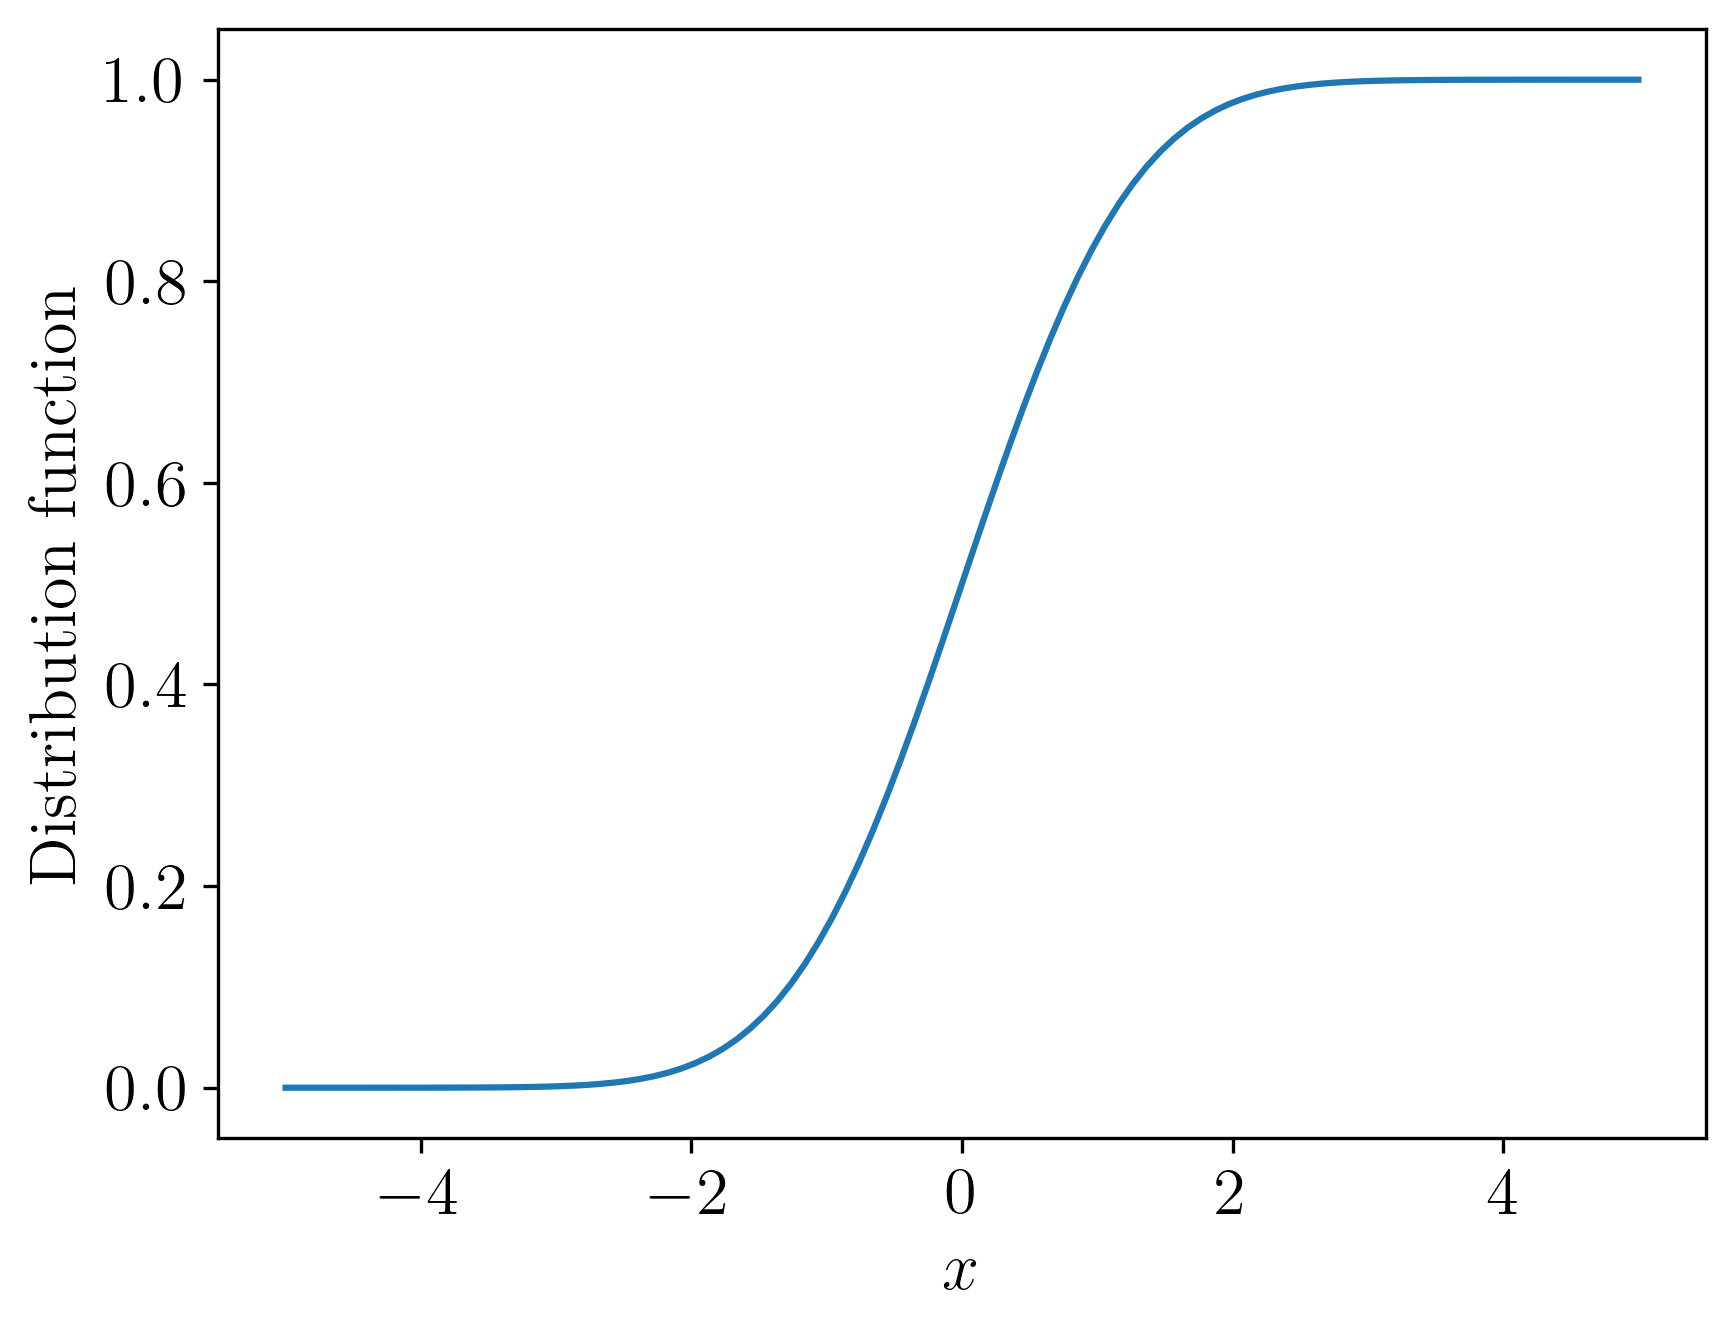
\includegraphics[width=.9\linewidth]{./Section/Grundlegende Begriffe/Verteilungsfunktion Normal.png}
\vspace*{-.3\baselineskip}
\caption{\centering Verteilungsfunktion einer $\Nor(0, 1)$-Verteilung}
\vspace*{-.3\baselineskip}
\end{center}
\end{figure}
\end{minipage}
\begin{minipage}{0.5\linewidth}
\begin{figure}[H]
\begin{center}
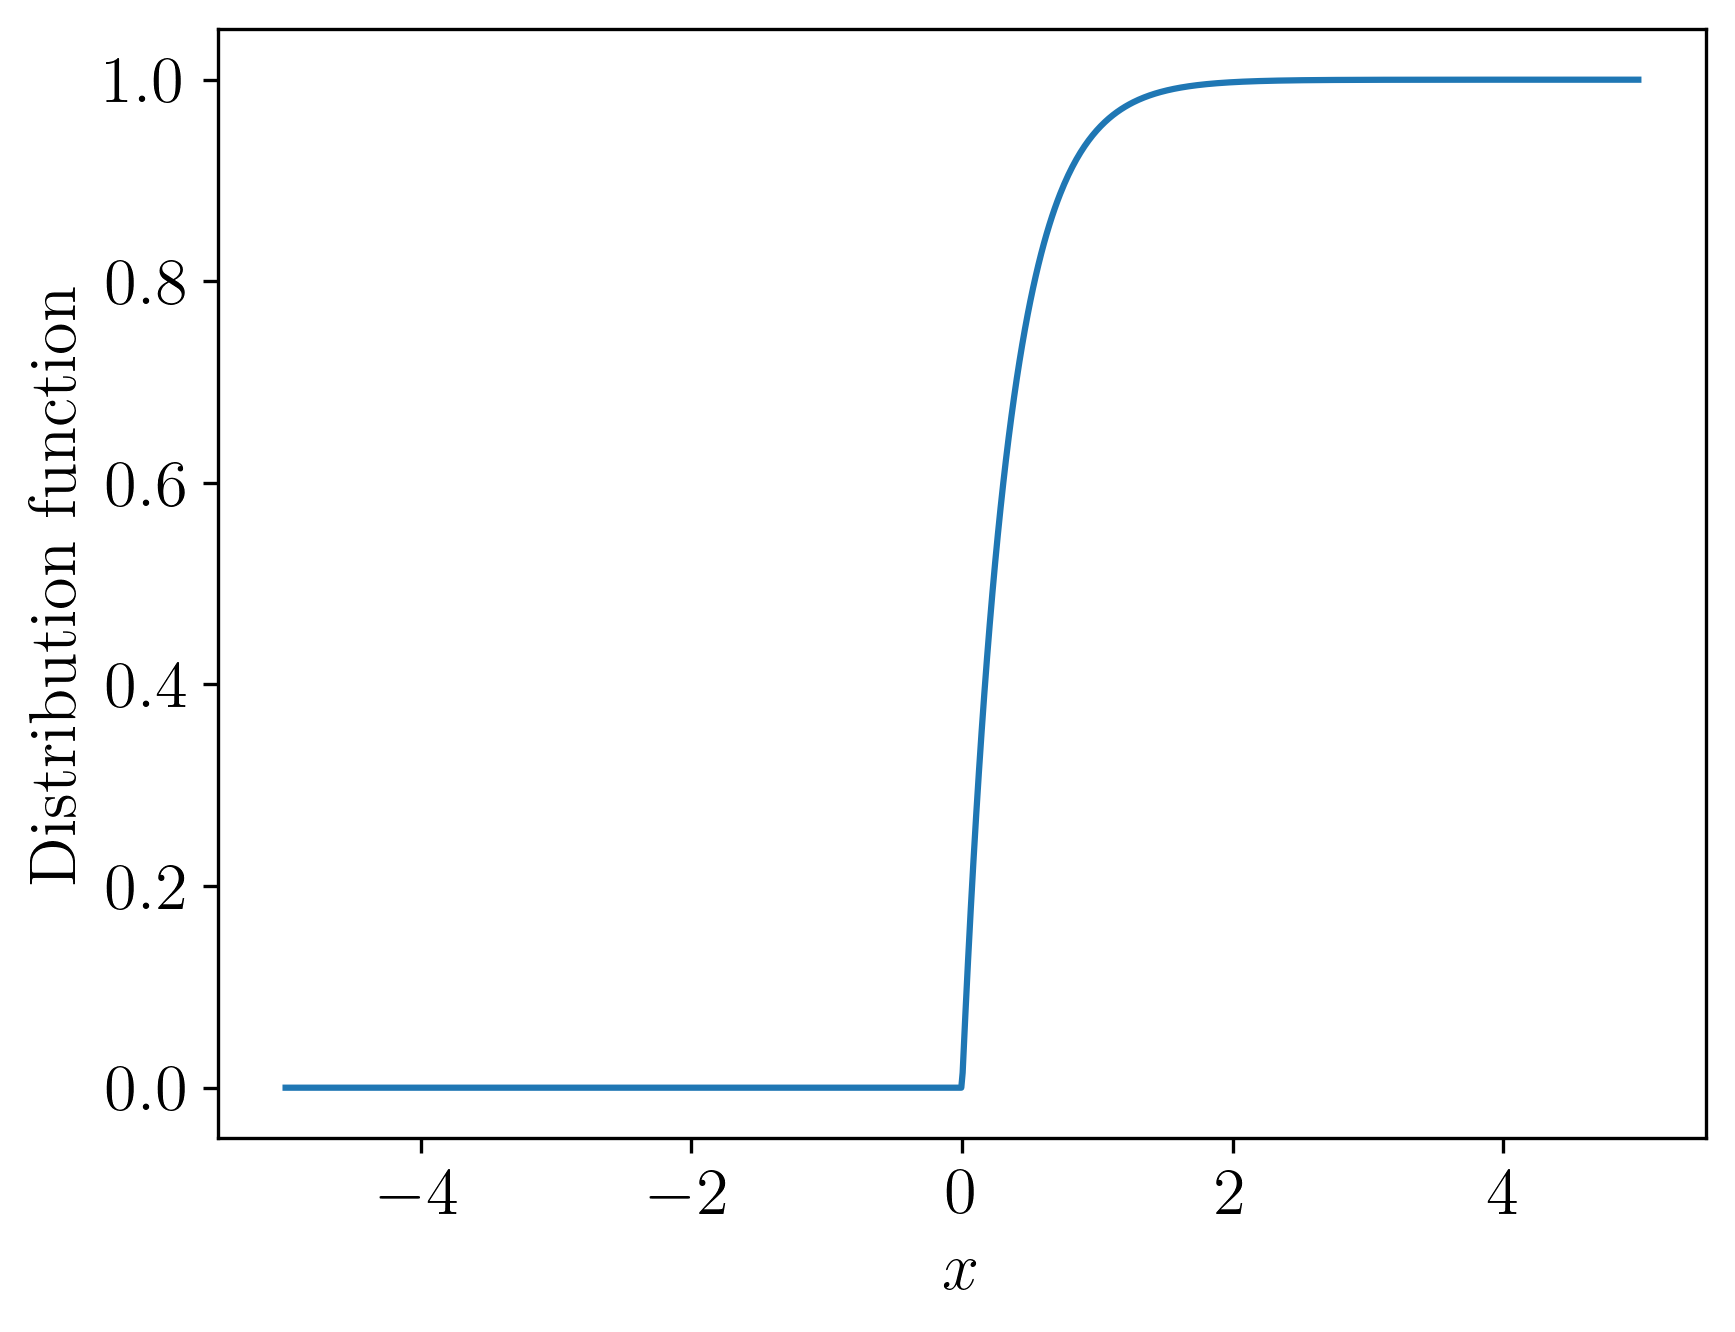
\includegraphics[width=.9\linewidth]{./Section/Grundlegende Begriffe/Verteilungsfunktion Exponential.png}
\vspace*{-.3\baselineskip}
\caption{\centering Verteilungsfunktion einer $\Exp(3)$-Verteilung}
\vspace*{-.3\baselineskip}
\end{center}
\end{figure}
\end{minipage}

Wir sehen bei allen Verteilungsfunktionen, dass sie nur Werte aus $[0, 1]$ annehmen und insbesondere die Grenzwerte $0$ und $1$ für $x \rightarrow -\infty$ und $x \rightarrow \infty$ haben. Außerdem sehen wir, dass Verteilungsfunktionen monoton wachsend sind. Bei der Bernoulli- und Binomialverteilung sehen wir deren stückweise stetige Natur. Die stetigen Verteilungen sind sogar stetig. Dies sind genau die Aussagen, die wir im \hyperlink{Satz:EigVertFun}{\blue{Satz über die Eigenschaften der Verteilungsfunktion}} gezeigt haben.
\end{Beispiel}
